%%
%% This is file `sample-sigconf.tex',
%% generated with the docstrip utility.
%%
%% The original source files were:
%%
%% samples.dtx  (with options: `sigconf')
%% 
%% IMPORTANT NOTICE:
%% 
%% For the copyright see the source file.
%% 
%% Any modified versions of this file must be renamed
%% with new filenames distinct from sample-sigconf.tex.
%% 
%% For distribution of the original source see the terms
%% for copying and modification in the file samples.dtx.
%% 
%% This generated file may be distributed as long as the
%% original source files, as listed above, are part of the
%% same distribution. (The sources need not necessarily be
%% in the same archive or directory.)
%%

%% The first command in your LaTeX source must be the \documentclass command.
\documentclass[sigconf]{acmart} 
\settopmatter{printacmref=false}
\usepackage{hyperref}  

%%
%% \BibTeX command to typeset BibTeX logo in the docs
\AtBeginDocument{%
  \providecommand\BibTeX{{%
    \normalfont B\kern-0.5em{\scshape i\kern-0.25em b}\kern-0.8em\TeX}}}
\setcopyright{none}
\hyphenation{De-zi-mal-tren-nung}
\renewcommand
\footnotetextcopyrightpermission[1]{}


%%
%% Submission ID.
%% Use this when submitting an article to a sponsored event. You'll
%% receive a unique submission ID from the organizers
%% of the event, and this ID should be used as the parameter to this command.
%%\acmSubmissionID{123-A56-BU3}

%%
%% The majority of ACM publications use numbered citations and
%% references.  The command \citestyle{authoryear} switches to the
%% "author year" style.
%%
%% If you are preparing content for an event
%% sponsored by ACM SIGGRAPH, you must use the "author year" style of
%% citations and references.
%% Uncommenting
%% the next command will enable that style.
%%\citestyle{acmauthoryear}

%%
%% end of the preamble, start of the body of the document source.
\begin{document}\setlength\emergencystretch{1.5em}

%%
%% The "title" command has an optional parameter,
%% allowing the author to define a "short title" to be used in page headers.
\title{Dokumentation ITIL - Qualitätssicherung}

%%
%% The "author" command and its associated commands are used to define
%% the authors and their affiliations.
%% Of note is the shared affiliation of the first two authors, and the
%% "authornote" and "authornotemark" commands
%% used to denote shared contribution to the research.

\author{Lara Krautmacher}
\email{lara.krautmacher@student.reutlingen-university.de}
\affiliation{%
  \city{Matrikelnummer: 123425}
  \institution{\\Informatik: IT-Management}
  \streetaddress{Alteburgstraße 150}
  \city{72762 Reutlingen}
  \state{Baden-Württemberg}
  \country{Deutschland}  
}
\author{René Wiskow}
\email{rené.wiskow@student.reutlingen-university.de}
\affiliation{%
  \city{Matrikelnummer: 801861}
  \institution{\\Informatik: IT-Management}
  \streetaddress{Alteburgstraße 150}
  \city{72762 Reutlingen}
  \state{Baden-Württemberg}
  \country{Deutschland}
}



\author{Elena Kirsch}
\email{elena.kirsch@student.reutlingen-university.de}
\affiliation{%
  \city{Matrikelnummer: 763207}
  \institution{\\Informatik: IT-Management}
  \streetaddress{Alteburgstraße 150}
  \city{72762 Reutlingen}
  \state{Baden-Württemberg}
  \country{Deutschland}
}


%%
%% By default, the full list of authors will be used in the page
%% headers. Often, this list is too long, and will overlap
%% other information printed in the page headers. This command allows
%% the author to define a more concise list
%% of authors' names for this purpose.


%%
%% The abstract is a short summary of the work to be presented in the
%% article.
\begin{abstract}
Qualitätssicherung spielt eine zentrale Rolle in jedem Unternehmen.
Reibungslose Abläufe interner Prozesse sowie die Erfüllung
von Ansprüchen an ein Endprodukt werden durch die Qualitätssicherung
garantiert. Im Zuge dieser Seminararbeit wird
anhand eines Planspiels evaluiert inwieweit die IT Infrastructure
Library die Organisation und Durchführung einer effizienten Qualitätssicherung
unterstützt. Dazu wurde das fiktive Unternehmen
\textit{TopBlogAG}, bestehend aus fünf Arbeitsgruppen, gegründet, welches
als Zielsetzung die Erstellung einer Blogging-Platform hat. Die
Arbeitsgruppe Qualitätssicherung hat dazu verschiedene Teststrategien
sowie Schwachstellenanalysen durchgeführt. Durch die Definition
der Key Performance Indicators in der Service-Quality Policy
ist festgelegt, wann die Ziele des Qualitätssicherungsprozesses
erreicht sind. 
\end{abstract}

%%
%% The code below is generated by the tool at http://dl.acm.org/ccs.cfm.
%% Please copy and paste the code instead of the example below.
%%


%%
%% Keywords. The author(s) should pick words that accurately describe
%% the work being presented. Separate the keywords with commas.
\keywords{IT-Management,ITIL, Qualitätssicherung, Service Transition}

%% A "teaser" image appears between the author and affiliation
%% information and the body of the document, and typically spans the
%% page.
\settopmatter{printfolios=true}
%%
%% This command processes the author and affiliation and title
%% information and builds the first part of the formatted document.
\maketitle

\section{Einleitung - Elena}
Unternehmen sind bestrebt ihre Prozesse, Produkte oder auch Dienstleistungen durch Frameworks und Zertifizierungen zu verbessern und deren Qualität stetig zu steigern. 
Die Qualität von Produkten ist entscheidend wie gut sich ein Unternehmen in dem jeweiligen Markt etablieren kann. Im allgemeinen Sprachgebrauch steht das Wort \textit{Qualität} für die Beschaffenheit oder Eigenschaft einer Sache oder Person \footnote{https://www.duden.de/rechtschreibung/Qualitaet, Zugriff: 12.06.2021} In der Wirtschaft bezeichnet Qualität den Wert oder die Güte einer Sach- oder Dienstleistung aus Sicht des Anwenders/der Anwenderin\footnote{http://wirtschaftslexikon24.com/d/qualitaet/qualitaet.htm, Zugriff: 12.06.2021}. Die ISO 9000:2015 beschreibt, dass  \begin{quote} die Qualität der Produkte und Dienstleistungen   einer    Organisation durch die Fähigkeit bestimmt wird, Kunden zufrieden zu stellen sowie durch die  beabsichtigte  und  unabsichtliche  Auswirkung  auf relevante interessierte Parteien ~\cite[S.~10]{DeutscheGesellschaftfurQualitat.November2015}\end{quote}. Ergänzt wird die Definition mit der Beschreibung, dass \begin{quote} die Qualität von Produkten und Dienstleistungen nicht nur deren vorgesehene Funktion und Leistung umfasst, sondern auch ihren wahrgenommenen Wert und Nutzen für den Kunden~\cite[S.~10]{DeutscheGesellschaftfurQualitat.November2015}\end{quote}.
Damit Frameworks die Verbesserung von Qualität eines Unternehmens und dessen Produkte, Dienstleistungen und Prozesse unterstützen können, müssen die Organisationen Richtlinien verfassen, die die Werte, Regeln und gewünschten Verhaltensweisen im Unternehmen festlegen. Um die Ziele einer Richtlinie zu erreichen, wird die Disziplin des Managements hinzugezogen, die ineinandergreifende Funktionen der Formulierung der Unternehmenspolitik sowie Organisation, Planung, Steuerung und Steuerung der Ressourcen eines Unternehmens umfasst\cite{KarlMichaelGauch.22.03.2021}. Für die Erweiterung auf den IT Bereich in Organisationen oder im Allgemeinen IT Unternehmen, wird das Management um das IT Management erweitert. Das IT Management ist im Groben für den professionellen Betrieb von großer Computersysteme zuständig \cite{KarlMichaelGauch.22.03.2021}. Indem das IT Management um den Bereich IT Service Management (ITSM) ergänzt wird, können verschiedene Handlungstätigkeiten in diesem Rahmen bearbeitet werden. Hierbei wurde im Jahr 2005 die ISO/IEC 2000 IT Service veröffentlicht, um einen Messbaren Qualitätsstandard zu erhalten \footnote{https://www.iso.org/standard/51986.html, Zugriff: 31.05.2021}. Durch ITSM stellen Organisationen sicher, dass ihre IT-Services so funktionieren, dass diese durch Benutzer*innen und das Unternehmen selbst genutzt werden können \footnote{https://www.ibm.com/cloud/learn/it-service-managementtoc-what-is-it-CCWD9gs4, Zugriff: 31.05.2021}. Im Allgemeinen handelt es sich bei ITSM um eine Reihe von Richtlinien und Praktiken, die die Implementierung, Bereitstellung und Verwaltung von IT-Services festschreibt. Dabei liegt der Fokus auf den erklärte Bedürfnissen der Endnutzer*innen und den erklärten Zielen des Unternehmens.
Für die Implementierung und Dokumentation von ITSM dient das
am weitesten verbreitete Best-Practice-Framework, die Information Technology Infrastructure Library (ITIL)\footnote{https://www.ibm.com/cloud/learn/it-service management toc-what-is-it-CCWD9gs4}. Das Framework ITIL bietet den Unternehmen die Rahmenbedingungen, um die Services optimal auf die Anforderung aus dem Business abzustimmen und regelmäßig auf die beste Unterstützung der Geschäftsprozesse zu überprüfen \cite{Beims.2015}. ITIL wird bei seiner Anwendung in fünf Lebenszyklusphasen eingeteilt. Die verschiedenen Lebenszyklusphasen sind gegliedert nach welchen Objekten sich die jeweilige Phase gerade richtet, welche Schlüsselkonzepte verwendet, welche Prozesse angewendet  und welche Modelle in dem Zyklus zugrunde gelegt werden. Zudem sind die jeweiligen Dokumente und Ergebnisse jeder Phase festgelegt. Innerhalb der Service Transition sowie der Continual Service Improvment spielt die Qualitätssicherung
eine wichtige Rolle. Somit müssen die in der Service Strategy identifizierten Services und Strategien in der Service Transition Phase getestet werden. Und auch die Ergebnisse aus der Service Design Phase wie zum Beispiel die Architekturen oder die Service-Level-Agreements müssen durch die Qualitätssicherung überprüft werden \cite{Beims.2015}. \\
Im Rahmen der Vorlesung IT-Management wurde die \textit{TopBlog AG} gegründet. Für den Aufbau der Organisation wurden fünf Arbeitsgruppen eingerichtet, die verschiedene Tätigkeitsfelder und Rollen im Rahmen von ITIL zu übernehmen hatten. Die dazu notwendigen theoretischen Hintergründe von ITIL im Allgemeinen sowie mit dem Fokus auf die Qualitätssicherung wird in \ref{chapter_theoretischeHintergünde} erläutert. Der genaue Rahmen, in dem das Framwork ITIL angewendet wird, beschreibt das Kapitel \ref{chapter_praktischedurchführung}  Praktische Durchführung. Die Reflektion des gesamten Projekts wird in Kapitel \ref{chapter_ReflektionDesProjekts} geschildert sowie ein Fazit in Kapitel \ref{chapter_Fazit}.

\section{Theoretische Hintergünde - Elena}
\label{chapter_theoretischeHintergünde}
ITIL ist toll

\subsection{ITIL}
\ref{chapter_theoretischeHintergünde} blablalkdshdoishdioedhe8ohzeourd \nameref{chapter_theoretischeHintergünde}

\subsection{Qualitätsicherung in ITIL - Lara}
Qualitätssicherung spielt im ITIL Framework eine zentrale Rolle.
Dies ist darauf zurückzuführen, dass ein Grundgedanke von ITSM
darin besteht die Qualität und Quantität von IT-Services zu planen,
überwachen und steuern [1]. An dieser Stelle wird beschrieben in
welchen Bereichen von ITIL Qualitätssicherung beachtet werden
muss.
ITIL Service Management ist in fünf Kernbereiche aufgeteilt, Service
Strategy, Service Design, Service Transition, Service Operation,welche
zeitlich nacheinander ablaufen, und Continual Service Improvement
(CSI), welcher paralell zu den anderen Teilbereichen kontinuierlich
bespielt wird. Qualitätssicherung findet dabei in den größten Teilen
im Bereich CSI statt, muss jedoch auch in den anderen Teilbereichen
immer mit betrachtet werden. Bei \textit{Service Strategy} , \textit{Service Design},
\textit{Service Transition}, \textit{Service Operation} wird Qualitätsmanagement
in die Prozesse integriert, indem bei der Planung zunächst betrachtet
wird, welche Qualitätsanforderungen an den Service bestehen,
sodass dem Nutzer einen Mehrwert im Produkt erkennt. Diese Anforderungen
werden anschließend in messbaren Kennzahlen (KPI’s)
quantifiziert. Die Definition der KPI’s, die gemessen werden sollen
bilden die Grundlage für den CSI-Improvement Prozess. In diesem
werden zur Verbesserung des Services sieben Phasen durchlaufen.

\subsubsection{Qualitätssicherung Allgemein}
bdbsjd

\subsubsection{Continuous Service Improvment}

\subsubsection{Testing}
Der Testing Prozess stellt die Einhaltung des Vertrags, welcher
mit dem Kunden über die Qualitätsanforderungen abgeschlossen
wird, sicher. Der Nutzen des Kunden steht daher im Mittelpunkt. Es
kann dabei zwischen zwei verschiedenen Kategorien unterschieden
werden: Die \textit{Utility} (Nützlichkeit) und die \textit{Warranty} (Garantie) \cite{Beims.2015}. Die Utility befasst sich dabei direkt mit den vom Kunden erwarteten
Services, während die Warranty die Verfügbarkeit dieser
Services ins Auge fasst. Aus diesen beiden Kategorien leitet sich die
Notwendigkeit ab, zum einen das Produkt selbst zu Testen, als auch
die Strukturen, welche den Nutzen des Produkts ermöglichen. Dazu
gehören unter anderem interne Services, sowie das Deployment-
Umfeld. Die Tests zielen dabei darauf ab, Fehler zu identifizieren und zu evaluieren ob vom Kunden gestellte Anforderungen wie gewünscht
erfüllt wurden. Final müssen die erhobenen Ergebnisse an
die verantwortliche Personen gemeldet werden, um Fehlerquellen
möglichst schnell zu beheben. Da in vielen Bereichen getestet werden
muss, um diese Kriterien sicherzustellen, ist eine umfassende
Teststrategie unabdingbar. 

Bei der Entwicklung einer geeigneten Teststrategie wurde sich an das Service V-Modell gehalten, welches in Abbildung \ref{fig:vmodell} dargestellt ist. Dieses definiert zu jedem Design- bzw. Entwicklungsschritt der einzelnen Services eine passenden Test. Dabei kann dieser Prozess in fünf Abschnitte unterteilt werden: \\

Der \textit{Component Test} wird parallel zur eigentlichen Service Entwicklung definiert. Dieser prüft, ob die einzelnen Komponenten, bzw. eine Gruppe an Komponenten, die geforderte Spezifikationen erfüllt. Es wird die direkte technische Umsetzung der Services getestet. Der \textit{Release Package Test} testet anschließend, ob die erstellten Services fehlerfrei bereitgestellt (deployed) werden können. Der \textit{Operational Readiness Test} bezieht sich auf die Ressourcen, welche vorhanden sein müssen, um den Service bereitzustellen. Damit sind nicht nurtechnische, sondern auch Humanressourcen gemeint. Es wird also genau so danach gefragt, ob genügend Speicher vorhanden ist, wie auch, ob der Support für den jeweiligen Service geleistet werden kann. Der \textit{Acceptance Test} erfolgt im direkten Zusammenspiel mit dem Kunden. Hier wird sichergegangen, dass der Service alle gestellten Kundenanforderungen zufriedenstellend erfüllt. An letzter Stelle steht die \textit{Service Validierung}. Dazu wird geprüft, ob der Service alle Verträge einhält. 

\begin{figure}[th]
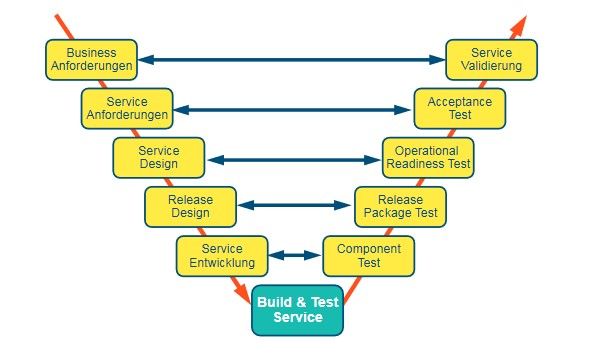
\includegraphics[width=\columnwidth]{V-Modell.jpg}
\caption{Service V-Modell \cite{Beims.2015} }
\label{fig:vmodell}
\end{figure}

\section{Praktische Durchführung}
\label{chapter_praktischedurchführung}
Macht Spaß

\subsection{Qualitätssicherung im Planspiel - Lara}
Macht Spaß

\subsubsection{Service Quality Policy. Definition Key Performance Indicators und Testing der KPI’s}

\subsubsection{Prozessdefinition zur Qualitätssicherung.}
Hier kommt ein Text

\subsection{Teststrategie-Rene}
\begin{itemize}
\item Beim Entwickeln einer Teststrategie an das Service V-Modell gehalten
\item Einzelne Tests dementsprechend direkt aus Entwicklungs/Design- Phasen abgeleitet
\item V-Modell in fünf Phasen
\end{itemize}

\textbf{Component Test}
\begin{itemize}
\item Erfüllt Komponente(ngruppen) Spezifikation?
\item ZB: Funktioniert Anmeldung etc.
\item Mit Entwicklern abgesprochen und Plan erstellt (Gantt)
\item Bezieht sich direkt auf die Implementation, bzw die Umsetzung der technischen Anforderungen
\item Getestet wurde die Implementierung des Blogging Portals
\item Dazu wurden zunächst die Annahme- bzw Abnahmekritierien aus den Anforderungen des Business Teams abgeleitet
\item Als nächstes wurden mögliche Schwachstellen identifiziert und Tests in Hinblick auf diese durchgeführt
\item Jedem Test wurde außerdem eine Priorität zugeordnet - Weiterhin wurde der interne Service des Service Desks, das Redmine Portal, getestet. Hier wurde ähnlich vorgegangen
\end{itemize}
\textbf{Release Package Test}
\begin{itemize}
\item Release- und Deployment Manager verantwortlich?
\item Funktionieren Release Optionen? Funktioniert Deployment?
\end{itemize}
\textbf{Operational Readiness Test}
\begin{itemize}
\item Sind wir in der Lage den Service so zu betreiben wie der Kunde es erwartet? Warranty
\item Fähigkeiten?
\item Ressourcen? (iT Operations)
\item Mitarbeiter?
\item Support organisiert? (Service Desk)
\end{itemize}
\textbf{Acceptance Test}
\begin{itemize}
\item Erfolgt mit Kunden
\item Service Abnahme wird mit Kunden durchgegangen (Business
Team)
\end{itemize}
\textbf{Service Validierung}
\begin{itemize}
\item Validierung der Angebote und Verträge
\item Werden Verträge eingehalten?
\end{itemize}

\subsection{Testplanung und -durchführung - Elena}
Excel

\section{REFLEKTION DES PROJEKTS}
\label{chapter_ReflektionDesProjekts}
Testen ... 

\section{FAZIT - RENE }
\label{chapter_Fazit}



%%
%% The next two lines define the bibliography style to be used, and
%% the bibliography file.
\bibliographystyle{ACM-Reference-Format}
\bibliography{itmanagement.bib}



\end{document}
\endinput
%%
%% End of file `sample-sigconf.tex'.
